\documentclass[10pt]{article}
\usepackage{graphicx}
\usepackage{longtable}
\usepackage{diagbox}
\begin{document}

\section{Data Analysis}

We transform the data from time series to stationary data using a flattening process. Random forests do not handle time series very well. Had we not transformed the data we would have had to worry about how the training and testing subsets were selected to ensure that future data is not used to predict past data. In addition, a decision tree cannot split on a non repeating independent variable such as time to produce any useful results.

The below table lists what columns are removed, and how other columns are transformed.


\subsection{Testing}
Since the Kaggle provided test data does not include the true classifications, we flatten the training set on all months save for the last month: 2016-5. The product classifications from 2015-1 to 2016-4 is used as our true predictor variables for each customer.

\subsection{Data Preprocessing}

\begin{longtable}{p{3cm}p{5cm}p{5cm}p{3cm}}
Column Name & Description & How To Flatten &  \\
fecha\_dato & The table is partitioned for this column & Remove in flattening &  \\
ncodpers & Customer code & Keep as key in flattening &  \\
ind\_empleado & Employee index: A active, B ex employed, F filial, N not employee, P pasive & Drop, since there are 13,576,218 NAs which is a huge proportion in the whole data set &  \\
pais\_residencia & Customer's Country residence & Use mode to fill NAs and flattening&  \\
sexo & Customer's sex & Use mode to clean the data and flattening&  \\
age & Age & Use max/final age for each customer. Outliers were moved to the median according to different age range &  \\
fecha\_alta & The date in which the customer became as the first holder of a contract in the bank & Shouldn't change &  \\
ind\_nuevo & New customer Index. 1 if the customer registered in the last 6 months. & Drop, since we have fecha\_alta &  \\
antiguedad & Customer seniority (in months) & Drop, since we have fecha\_alta &  \\
indrel & 1 (First/Primary), 99 (Primary customer during the month but not at the end of the month) & Drop, since we have indrel\_1mes &  \\
ult\_fec\_cli\_1t & Last date as primary customer (if he isn't at the end of the month) & Drop, since we have indrel\_1mes &  \\
indrel\_1mes & Customer type at the beginning of the month ,1 (First/Primary customer), 2 (co-owner ),P (Potential),3 (former primary), 4(former co-owner) & Use mode &  \\
tiprel\_1mes & Customer relation type at the beginning of the month, A (active), I (inactive), P (former customer),R (Potential) & Drop, since we have indrel\_1mes, activity index &  \\
indresi & Residence index (S (Yes) or N (No) if the residence country is the same than the bank country) & Drop, since we have pais\_residencia &  \\
indext & Foreigner index (S (Yes) or N (No) if the customer's birth country is different than the bank country) & Drop, since we have pais\_residencia &  \\
conyuemp & Spouse index. 1 if the customer is spouse of an employee & Drop, since too many NA &  \\
canal\_entrada & channel used by the customer to join & Drop, since too many NA &  \\
indfall & Deceased index. N/S & Drop, since we are dropping deceased custos &  \\
tipodom & Addres type. 1, primary address & Drop, we assume it won't matter &  \\
cod\_prov & Province code (customer's address) & Use mode &  \\
nomprov & Province name & Drop, since we have cod\_prov &  \\
ind\_actividad\_cliente & Activity index (1, active customer; 0, inactive customer) & Length of most recent inactive period \& how long ago that period was &  \\
renta & Gross income of the household & Use mean, fill NAs by median household income of different province &  \\
segmento & segmentation: 01 - VIP, 02 - Individuals 03 - college graduated & Use mode \& last &  \\
ind\_ahor\_fin\_ult1 & Saving Account & Timing: Months from fecha\_alta until first fecha\_dato in which product is purchased \& Length: Use sum &  \\


\end{longtable}

\section{Method}

\paragraph{Random Forest}
We use a random forest model with 100 trees. A RF model uses decision trees as weak predictors of the response variable to produce a strong predictor in the random forest. Each tree is produced on a random subset of samples with replacement and would otherwise suffer from over fitting and high variance. At each split a random subset of features without replacement is used to find the best split. Each tree produces a classification and the mode of the classifications becomes the forest's overall classification for the sample. However for our model, sklearn instead averages the probability of predicting a class across all trees.\cite{rnSKlearn}  The out of bag samples for each tree is used to test the tree and provide an unbiased estimator of the classification error.\cite{rnLeo} 

\paragraph{The Decision Tree}
Each split is made with respect to a random subset of features. The optimal split is chosen to minimize the impurity of the node being split on. The Gini impurity function is a common function to use. In all cases the goal is to split such that samples are grouped together by label.

\paragraph{Why did we choose a random forest?}

Random forests scale very well with large input sizes. The bagging process results in a strong predictor over all the trees. The random forest can also handle our categorical variables directly so we will not have to generate dummy variables for the categories. Additionally, the random forest supports multi-label classification so we don't have to separately fit model for each response variable.

\section{Results}

\subsection{Forest Tuning}

We tested the forest with varying number of trees and maximum depth. As expected, accuracy increased with tree size and depth. Ultimately we chose a tree size of 100 and maximum depth of 100.
\begin{table}[h]
    \centering
    \begin{tabular}{|c|c|c|c|}
        \hline 
        \backslashbox{Trees}{Depth} & 10 & 100 & \infty \\ 
        \hline 
        1 & 0.7434 & 0.8594  & 0.8594 \\ 
        10 & 0.8465 & 0.8956  & 0.8956 \\ 
        100 & 0.8518 & 0.9044  & 0.8921 \\ 
        \hline 
    \end{tabular} 
    \caption{Model Accuracy vs \# of Trees and Tree Depth}
    \label{tab:my_label}
\end{table}


\subsection{ROC for 100 trees with depth of 10}
\begin{center}
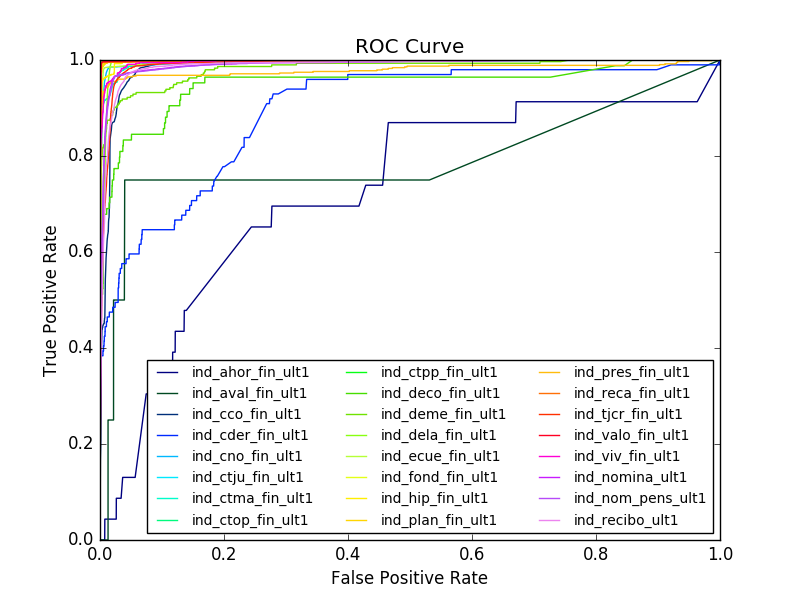
\includegraphics[width = 15cm]{ROC.png}
\end{center}

\subsection{Discussion}

As expected the benefits of the random forest can be seen in how our classification accuracy grows with the number of trees and tree depth. The very high accuracy for the forest of tree size one is most likely because most customers did not buy new products.


\subsection{Credits}

Charlton Lin: Created the flattening code and worked on feature engineering.
Qiaojuan Niu : Created the Random Forest model and code to clean the data.
Zoran Dabic: Wrote the subgroup report, worked on feature engineering, and ran the flatten and clean code to generate the final data sets.

\subsection{Reproduction}

Install Jupyter with the latest version of python. \\
Download the training and testing data from the Santander competition page. \\
Run fixData.py in the same directory as the training and testing data. This will generate fixed versions of the data sets. \\
Run flattenClean.py to create flattened versions of the fixed data sets. \\
Run the jupyter project RanForestForFlat.ipynb \\

\begin{thebibliography}{9}
\bibitem{rnLeo} 
Breiman, Leo and Cutler, Adele 
\textit{Random Forest}. 
\\\texttt{https://www.stat.berkeley.edu/~breiman/RandomForests/cc\_home.htm}
\bibitem{rnSKlearn} 
Scikit Learn,
\textit{Ensemble Methods}. 
\\\texttt{http://scikit-learn.org/stable/modules/ensemble.html}
\end{thebibliography}




\end{document}